% !TeX spellcheck = en_GB

	In this chapter we are going to explain the final models of the work and the preparation of the input data to feed these models. For the different solutions, we have used the algorithms previously explained in the models section \ref{section:models}. Below, it can be found a list which includes the 6 implementations:
	
	\begin{itemize}
		\item \acrshort{svm} classifier for multiclass classification
		\item \acrshort{svm} multiclass + \acrshort{svm} for a final binary classification
		\item \acrshort{lstm} for multiclass classification
		\item \acrshort{lstm} multiclass + \acrshort{svm} for a final binary classification
		\item \acrshort{cnn} for multiclass classification
		\item \acrshort{cnn} multiclass + \acrshort{svm} for a final binary classification
	\end{itemize}
	

\section{Input data preparation}
\label{section:input-data-preparation}

	For the proposed experiments, we have decided to build a small dataset formed by embeddings extracted form the .\textit{tfrecord} files that belong to 14 classes: half of them \textit{violent} and the other half, \textit{non-violent}. To find these, we first did a run on the simple user-interaction program that is explained in \ref{subsection:violent-classes}. \doubt{Putting ourselves in a gender-based violence victim's skin}, a total of 28 classes were selected . From this set, we picked 7 as the violent classes. The other 7 were chosen just by looking at the ontology.
	
	It is important to mention that this small dataset is composed by samples with just one label assigned. As explained before in \ref{section:audioset}, the database is unbalanced. Some of the most appropriated classes to be considered violence are really little populated. When doing the selection of categories, apart from paying attention to the own meaning of the class, we also checked the number of samples. For the non-violent type, this was not a problem, since we took some of the most-populated labels. However, in the violent case, we had to deal with the condition of representing violence and also having enough observations. So, due to these limitations, we could not obtain a set naturally balanced. In table \ref{table:7}, it is shown the 14 labels that were selected divided in violent and non-violent. In figure \ref{fig:mesh14}, a bar plot shows the number of samples obtained per class right after the selection. \todo{Include description of classes?}
	
	\begin{table}[ht]
		\centering
		\begin{tabular}{|| m{7em} | m{7em} ||}
			\hline
			\textbf{Violent} & \textbf{Non-violent} \\
			\hline\hline
			Baby cry, infant cry & Printer \\
			\hline
			Slap, smack & Music \\
			\hline
			Screaming & Speech \\
			\hline
			Machine gun & Vehicle \\
			\hline
			Breaking & Animal \\
			\hline
			Slam & Dishes, pots, and pans \\
			\hline
			Yell & Wind \\
			\hline
		\end{tabular}
	\caption{Relation of \textit{violent} and \textit{non-violent} selected classes}
	\label{table:7}
	\end{table}
	
	\begin{figure}[t]
		\centering
		\captionsetup{justification=centering}
		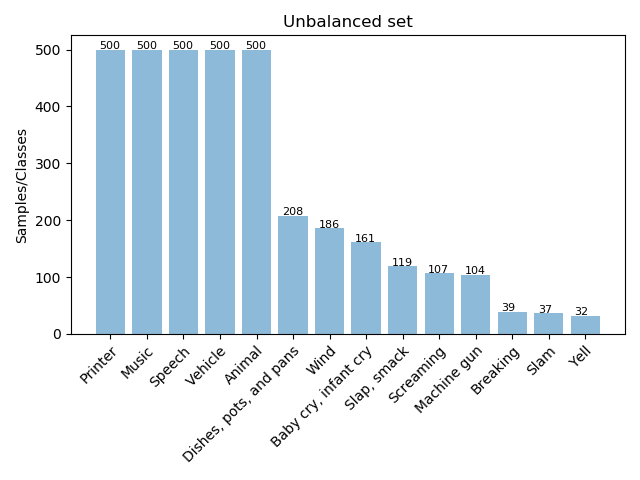
\includegraphics[scale=0.6]{samples-class-experiments}
		\caption{Bar plot that shows the number of samples for each of the selected classes. Clearly, the violent categories are much less populated than the others, that did not have to much any semantic criteria}
		\label{fig:mesh14}
	\end{figure}

	Some initial preprocessing were performed before passing the data to the different models. As mentioned in \ref{subsection:extracting-embeddings}, we had to deal with the zero-filling problem, which means that some of the rows of the embeddings matrices are completely zero because of the duration of the original video is less than 10s. As a solution, we decided to substitute the zero numbers in all the data with the machine epsilon\footnote{The machine epsilon value is considered the smallest value that satisfies $1 + \epsilon_{match} > 1$. It consists on the difference between one and the next closest number that is representable as a machine value \cite{Kaw}} value. 
	
	However, in the two models that use \acrshort{svm} for the multiclass classification a different solution was proposed. As it was explained in subsection \ref{label:svm}, this algorithm needs the input data matrix to be in the form [$number\ of\ samples\ \times\ number\ of\ features$], which differs from the originally shape of our data, [$number\ of\ samples\ \times\ number\ of\ seconds\ \times\ number\ of\ features$]. For this reason, we decided to reshape our data to the required form which resulted in a matrix of shape [$(number\ of\ samples\ \times\ number\ of\ seconds)\ \times\ number\ of\ features$]. With this conversion, instead of classifying full audio instances, the samples became the seconds of those instances. In order to remove zero data, we first checked the amount of zero-rows in every class. Since it was not very meaningful, we took them out of the dataset. 
	
	Once we had our data with all non-zero values, we needed to convert the set to balanced. First, for the classification task, we divided our data in train, validation and test subsets, using a 20\% for last one. Then, we decided to take out of the set half of the samples from the most populated classes \footnote{\textit{Speech}, \textit{Music}, \textit{Vehicle} and \textit{Animal}} from the train and validation sets, and generate new data for those with less observations by applying the data augmentation technique explained in subsection \ref{subsection:smote}. \doubt{This technique deduces a distribution for the given observations and generate synthetic samples within the distribution of each class until even the most populated category}. Just the train and validation set were subjected to this conversion, leaving the test set with the original embeddings. In figure \ref{fig:mesh15}, the subfigure (a) shows the distribution of data per class in the dataset for the case of the models that use \acrshort{svm} multiclass classifier. In subfigure (b), it is shown the distribution for the other four cases.
	
	\begin{figure}[ht]
		% Whole figure
		\captionsetup{justification=centering}
		\begin{subfigure}[b]{\textwidth}
			% Start with figure wav
			\centering
			\captionsetup{justification=centering}
			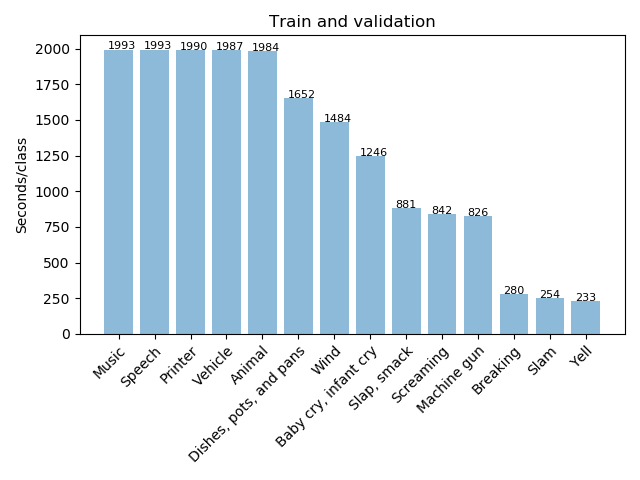
\includegraphics[width=0.5\linewidth]{tr_val_unbal_svm}%
			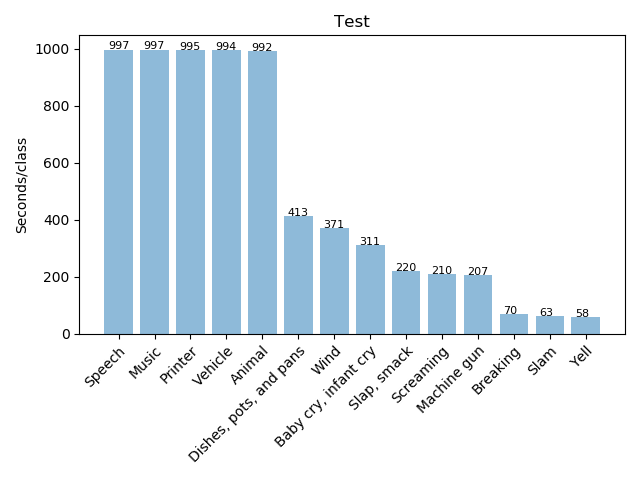
\includegraphics[width=0.5\linewidth]{tst_unbal_svm}
			\subcaption{This is the resulting subsets after downsampling the most populated classes and removing the zero-rows for the experiments that involve a SVM classifier}
		\end{subfigure}
		\vskip\baselineskip
		% Start with figure tfrecord
		\begin{subfigure}[b]{\textwidth}
			\centering
			\captionsetup{justification=centering}
			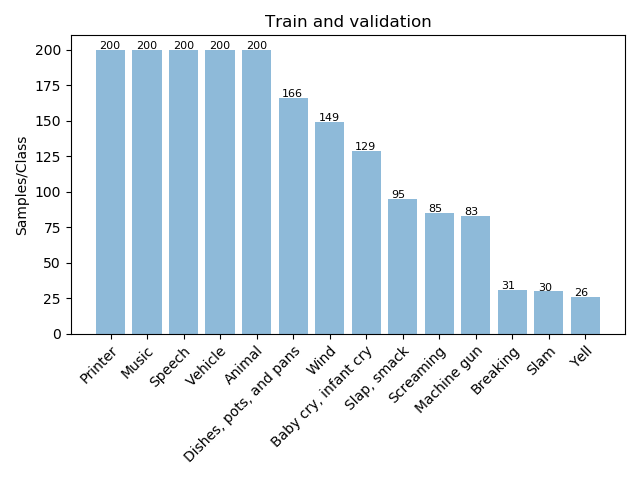
\includegraphics[width=0.5\linewidth]{tr_val_unbal}%
			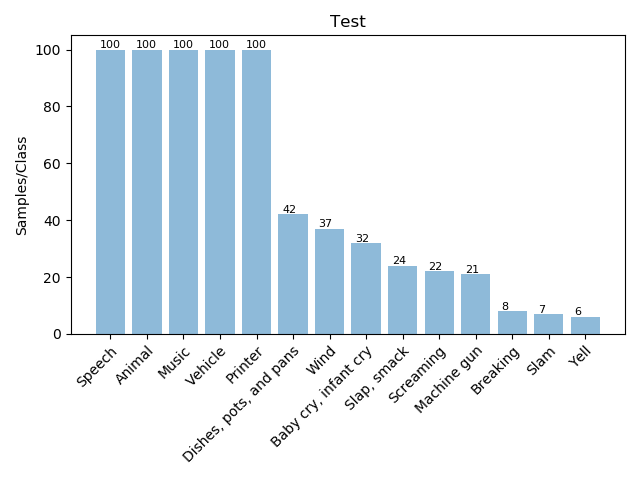
\includegraphics[width=0.5\linewidth]{tst_unbal}
			\subcaption{This is the resulting sets after downsampling the train and validation sets. The test set remains the same after the split}
		\end{subfigure}
		
		\caption{Number of observations for train, validation and test subsets used in the different experiments}
		\label{fig:mesh15}
	\end{figure}
	
	After these sets are obtained, the data augmentation technique \acrshort{smote} is applied. Finally, the shape input data for each of the experiments is shown in table \ref{table:8}
	
	\begin{table}[ht]
		\centering
		\begin{tabular}{|| m{7em} | m{10em} | m{10em} | m{10em} ||}
			\hline
			& \textbf{SVM multi and \acrshort{svm} + \acrshort{svm} binary} & \textbf{\acrshort{lstm} multi and \acrshort{lstm} + \acrshort{svm} binary} & \textbf{\acrshort{cnn} multi and \acrshort{cnn} + \acrshort{svm} binary}  \\
			\hline\hline
			\textbf{Train and validation} & 17645 (1993 per class) & 2800 (200 per class) & 2800 (200 per class) \\
			\hline
			\textbf{Test} & 6898 & 699 & 699 \\
			\hline                    
		\end{tabular}
		\caption{Train, validation and test set for different experiments}
		\label{table:8}
	\end{table}

\section{Implementations and results}

	For all the experiments, as mentioned above, the dataset was split by selecting a 20\% of the data for the testing procedure. The other part was divided into train and validation subsets with a \acrlong{kfold} technique, with 10 folds, which can also be called 10-fold cross-validation. A more detailed explanation about this resampling technique can be found in appendix \ref{appendix:kfold}. The average and standard deviation of the results for the different folds were obtained for training and validation. Then, a final measurement was performed for the test set. The way of checking the model performance was by finding the accuracy and confusion matrix, whose explanation can be found in appendix \ref{appendix:metrics}. For the cross-validation procedure, a matrix with the average values\footnote{In the average matrices, the results for each cell are shown just with one decimal in order to make a better and more comfortable visualization. However, the colour bar on the right of the plots must be taking into account since there might be some cells in which the value is $0.0$ but it is actually greater.} was obtained and also one for the standard deviation\footnote{In the standard deviation matrices the results are shown multiplied by $10^{2}$ in order to see the value in the different cells of the matrix} so the estimation of the model is represented for the corresponding subsets. Finally, a last evaluation of the model is performed by checking the accuracy just once with the test set. For this case, it is used the model that during the train and validation process let obtained a higher value of accuracy for the validation fold.
	
	As mentioned above, we have in total developed six final implementations. Three of them for a multiclass classification problem that consists of predicting the right label for each sample within the fourteen labels already explained. The other three are basically \acrshort{svm} binary classifiers that take as input the probabilistic output of the multiclass classifications. The purpose of these three is to adapt the model to the final objective of creating a model to distinguish between violent and non-violent events. For this classification.
	
		\begin{figure}[ht]
		% Whole figure
		\captionsetup{justification=centering}
		\begin{subfigure}[b]{\textwidth}
			% Start with figure wav
			\centering
			\captionsetup{justification=centering}
			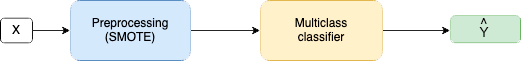
\includegraphics[scale=0.65]{multiclass-classifier}
			\caption{General model for the the three multiclass classification approaches.}
		\end{subfigure}
		\vskip\baselineskip
		% Start with figure tfrecord
		\begin{subfigure}[b]{\textwidth}
			\centering
			\captionsetup{justification=centering}
			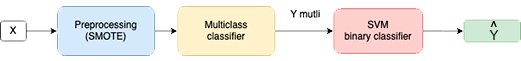
\includegraphics[scale=0.7]{mutli+svm-binary}
			\caption{Block diagram that shows the concatenation of multiclass classifier and the SVM binary classifier.}
		\end{subfigure}
		
		\caption{Confusion matrices for SVM multiclass classification for train and validation sets}
		\label{fig:mesh17}
	\end{figure}

	The output denoted as \textit{\^{Y} multi} corresponds to the predicted labels by the multiclass classifier. Then, this feeds the binary classifier that is trained with this new data. The split for this process is also 20\% for the test set and the rest is split into train and validation with a \acrshort{kfold} algorithm. Then, the model instance for which the best accuracy value was obtained in the validation set is used for the testing process.
	
\subsection{Implementation 1: \acrshort{svm} classifier for a multiclass classification}

	We decided to establish a benchmark by making a first experiment based on a \acrshort{svm} classifier that is used for a multiclass classification. In this case, we wanted to check the results of the performance of one of the most employed techniques in this filed different from \acrshort{nn}. It is true that this method is originally designed for binary problems but, as explained in \ref{subsection:svm}, we took advantage fo the multiclass algorithm. To define our model, we used mainly the default parameters. These includes of using a \acrshort{rbf} as a kernel. In this work, we have not investigated which type kernel could better fit our problem, however we found in the literature that the default option of \acrshort{rbf} is the most appropriated for real world applications \cite{Prajapati2010}. 
	
	Below, we can find the results for the different sets. In figure \ref{fig:mesh18}, the confusion matrices for the train and validation sets are shown. In figure \ref{fig:mesh19}, the confusion matrix for the evaluation on the test set is included. Finally, in the bar plot of figure \ref{fig:mesh20}, the accuracy values for the three sets are represented. For this case, the standard deviation is not shown for train and validation because it is zero when considering two decimals.
	
	\begin{figure}[ht]
		% Whole figure
		\captionsetup{justification=centering}
		\begin{subfigure}[b]{\textwidth}
			% Start with figure wav
			\captionsetup{justification=centering}
			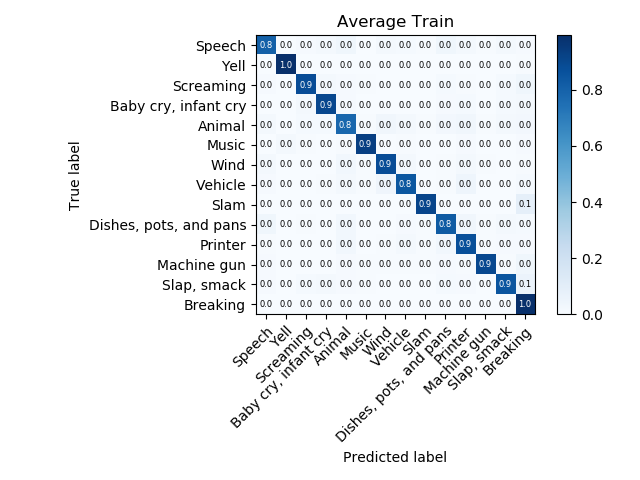
\includegraphics[width=0.6\linewidth]{svm-multi-cm-tr-av}%
			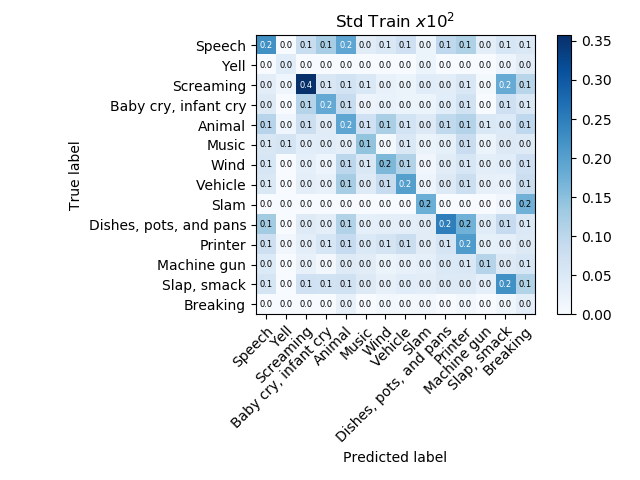
\includegraphics[width=0.6\linewidth]{svm-multi-cm-tr-std}
			\subcaption{Average and standard deviation for the train set}
		\end{subfigure}
		\vskip\baselineskip
		% Start with figure tfrecord
		\begin{subfigure}[b]{\textwidth}
			\captionsetup{justification=centering}
			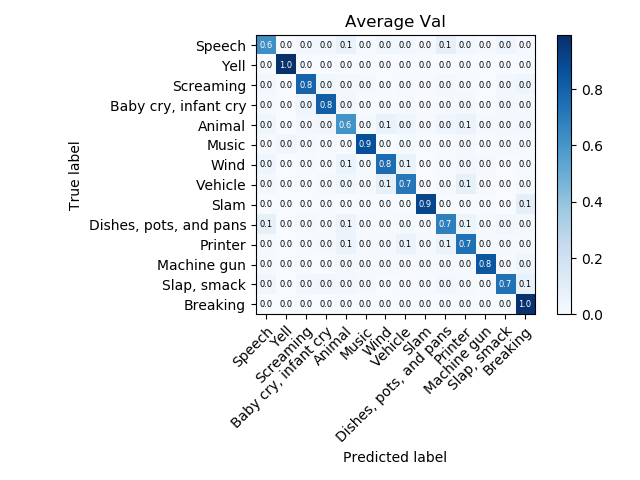
\includegraphics[width=0.6\linewidth]{svm-multi-cm-val-av}%
			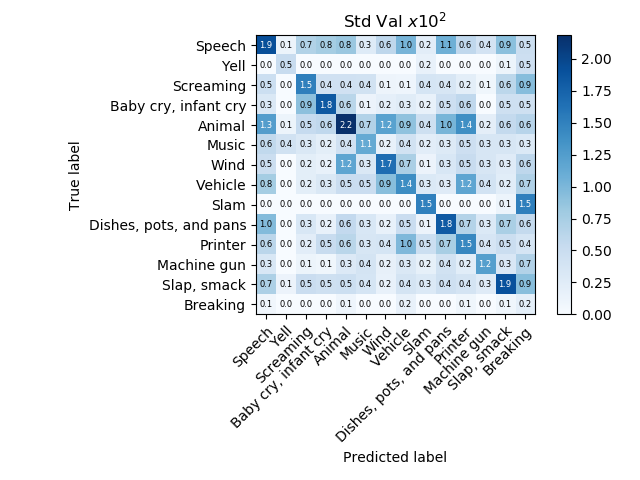
\includegraphics[width=0.6\linewidth]{svm-multi-cm-val-std}
			\subcaption{Average and standard deviation for the validation set}
		\end{subfigure}
		
		\caption{Confusion matrices for SVM multiclass classification for train and validation sets}
		\label{fig:mesh18}
	\end{figure}

	\begin{figure}[t]
		\centering
		\captionsetup{justification=centering}
		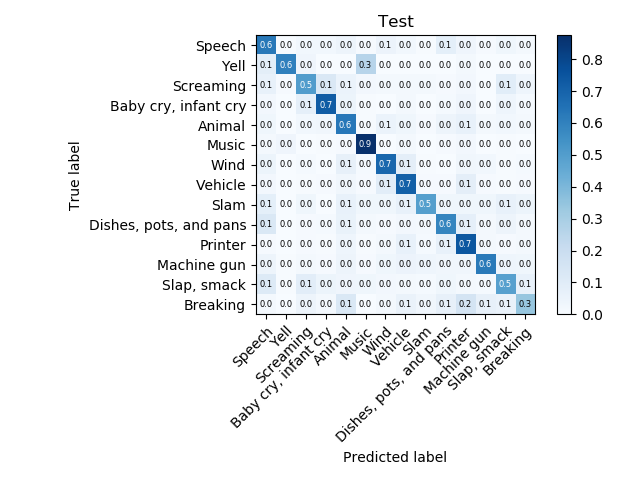
\includegraphics[width=0.7\linewidth]{svm-multi-cm-tst}
		\caption{Confusion matrix for the test set for the SVM multiclass classification}
		\label{fig:mesh19}
	\end{figure}

	\begin{figure}[t]
		\centering
		\captionsetup{justification=centering}
		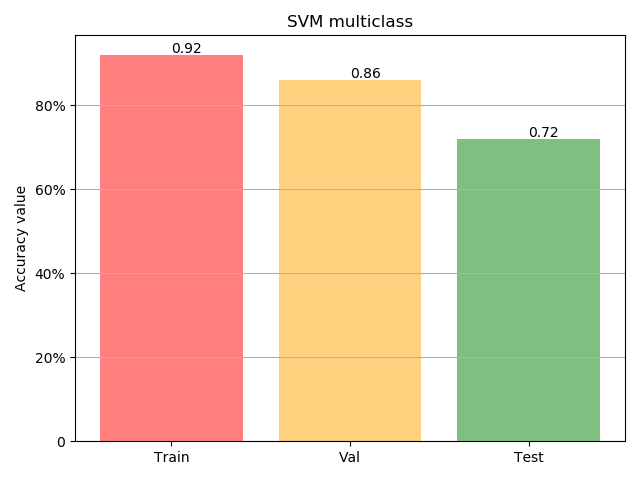
\includegraphics[width=0.7\linewidth]{svm-multierrorbar}
		\caption{Accuracy values for the three sets for the SVM multiclass classification}
		\label{fig:mesh20}
	\end{figure}

	As we can see, the values of the average values of accuracy are a $92\%$ for the training set, a $86\%$ for the validation and a $72\%$. This can also be appreciated in the average confusion matrices. The diagonal for the training and the validation stands out the other cells but they do not present a sense of overfitting due to they are not completely uniform. In the test results, we can see greater values in the true positive sections for the most populated classes explained above in section \ref{section:input-data-preparation}. This makes sense since the test set has more samples in these categories. We can consider a good result for this case. The accuracy of the final testing process is not much lower than the one obtained for the validation set. It would be a good option to populate more the violent labels, but we did not wanted to use synthetic data in the final evaluation.

\subsection{Implementation 2: \acrshort{svm} multiclass classification and \acrshort{svm} binary classification}

	Once we have trained the \acrshort{svm} multiclass classifier, we save the model for which the accuracy of the validation set in the cross-validation has a greater value. Then, it is incorporated to the previous stage of the preprocessing. So, it predicts the multiclass label for each value what can also be interpreted as it is converting the data to a new feature space before the binary classification.
	
	The results in accuracy and confusion matrices for the different evaluations can be found below. Figure \ref{fig:mesh23} includes the average confusion matrices for train and validations sets. Then, in figure \ref{fig:mesh24}, the confusion matrix for the test set is included. Finally, in figure \ref{fig:mesh25}, the accuracy values for the three sets are shown, with their perspective standard deviations.
	
	\begin{figure}[t]
		\centering
		\captionsetup{justification=centering}
		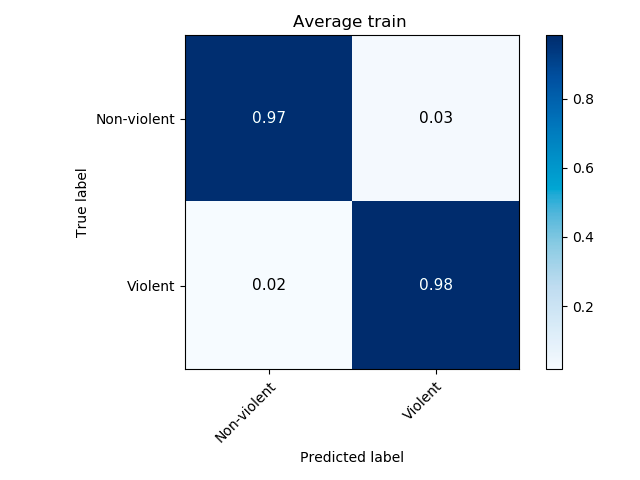
\includegraphics[width=0.6\linewidth]{svm-svm-cm-tr-av}%
		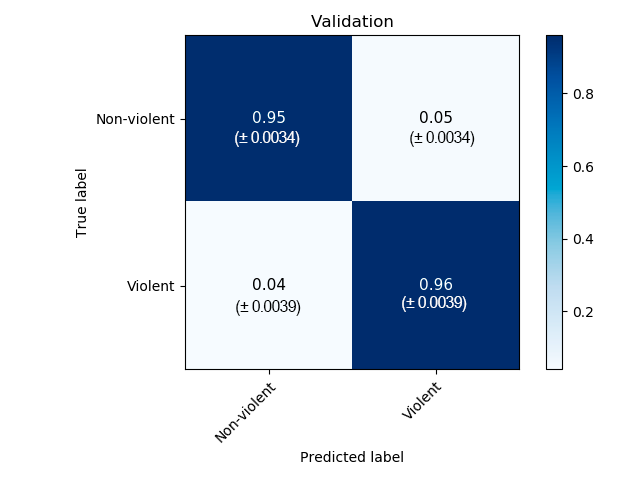
\includegraphics[width=0.6\linewidth]{svm-svm-cm-val-av}	
		\caption{Average confusion matrices for train and validation in the SVM multiclass + SVM binary classification}
		\label{fig:mesh23}
	\end{figure}
	
	\begin{figure}[t]
		\centering
		\captionsetup{justification=centering}
		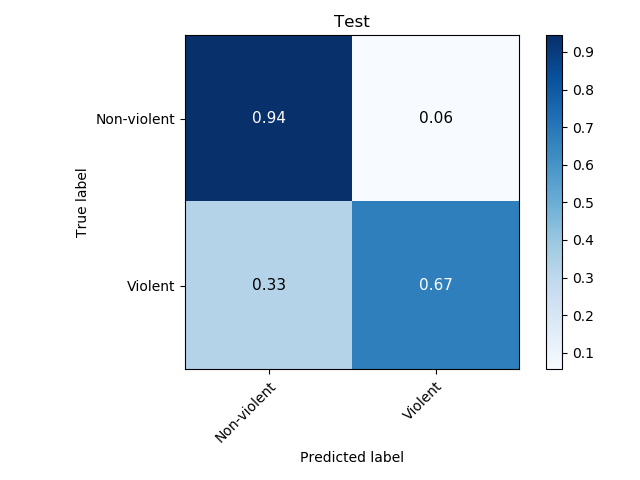
\includegraphics[width=0.7\linewidth]{svm-svm-cm-tst}
		\caption{Confusion matrix for the test set for the SVM multiclass + SVM binary classification}
		\label{fig:mesh24}
	\end{figure}
	
	\begin{figure}[t]
		\centering
		\captionsetup{justification=centering}
		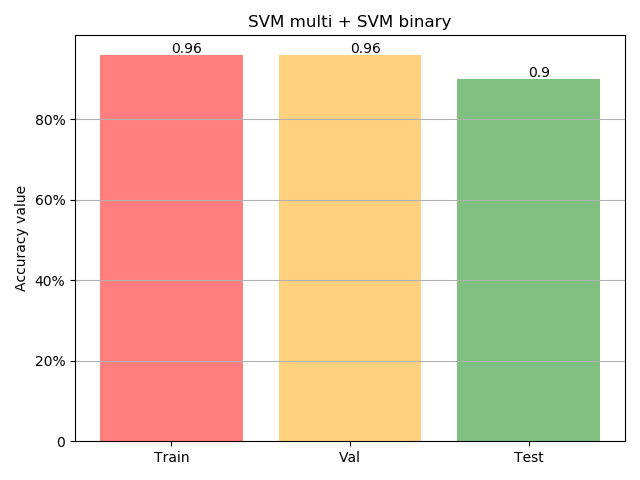
\includegraphics[width=0.7\linewidth]{svm-binaryerrorbar}
		\caption{Accuracy values for the three sets for the SVM multiclass + SVM binary classification}
		\label{fig:mesh25}
	\end{figure}

	In this performing model it is more important to pay attention to both metrics. In the accuracy bar plot, at first, it can be interpreted that the results are really good. This can be due to the elevated number of samples for a binary classification. Considering the test value of 91\%, we can see that the merit of the good performance is thank to the good classification of the non-violent observations, while the result on differentiating the violent classes is not as good since just the 60\% of the labels were correctly predicted. For the train and validation sets, the results are pretty good for both types, being a 98\% for both cases. Again, the fact of creating a big amount of the samples artificially for the training and validating parts is given a considerable difference in the results respect to the testing. However, this output also allows to see that with a more balanced test set the performance would be more even in the tree sets, as it happened with the multiclass task explained before, and that those observations which belong to the original embeddings show a satisfying outcome.
	
\subsection{Implementation 3: \acrshort{lstm} for multiclass classification}

	For this implementation we have decided to use a network composed by a total of three layers: two \acrshort{lstm} and a final \acrlong{fc} with a softmax activation function for the classification task. The first two \acrshort{lstm} layers are set with a dropout of 0.05 and a recurrent dropout of 0.35. For the first one, the number of units was set to 128, in order not to change the dimensions of its output. In the second layer, it was set to 32 layers so as to reduce the dimensionality before the final prediction in the dense layer. In figure \ref{fig:mesh26}, an schema of the model is shown.

	\begin{wrapfigure}{R}{0.4\textwidth}
		\centering
		\captionsetup{justification=centering}
		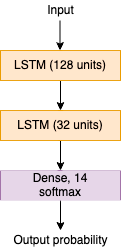
\includegraphics[scale=0.4]{lstm}
		\caption{Architecture for the LSTM multiclass classifier implementation}
		\label{fig:mesh26}
	\end{wrapfigure}
	
	The function minimized in the process was the categorical cross-entropy, which is a common way to evaluate multiclass classification problems. A more detailed explanation of this function can be found in appendix \ref{appendix:categorical-cross-entropy}. With respect to the training process, a number of 50 epochs were used and also a batch size of 32 samples \footnote{When training a machine learning model, an optimization algorithm, usually \acrshort{sgd}, is in charge of updating the internal parameters so a good performance is achieved and the loss function can be minimized. The epochs is a hyperparameter that establishes how many times the learning algorithm pass through the entire train set in the training process. The batch size is the one that defines the number of observations the algorithm works through before assigns the internal parameters an updated value \cite{Browniee2018a}}. \todo{remove from footnote} Also, a \acrshort{nadam} optimizer was used and a learning rate of $2e^{-3}$.
	
	Below, the results for the classification are included. In figure \ref{fig:mesh27}, the average and standard deviation matrices for the train and validation sets are shown. Then, in figure \ref{fig:mesh28}, the confusion matrix for the testing process is included. In figure \ref{fig:mesh29}, a bar plot shows the accuracy for every set with their standard deviation values.
	
		\begin{figure}[ht]
		% Whole figure
		\captionsetup{justification=centering}
		\begin{subfigure}[b]{\textwidth}
			\centering
			% Start with figure wav
			\captionsetup{justification=centering}
			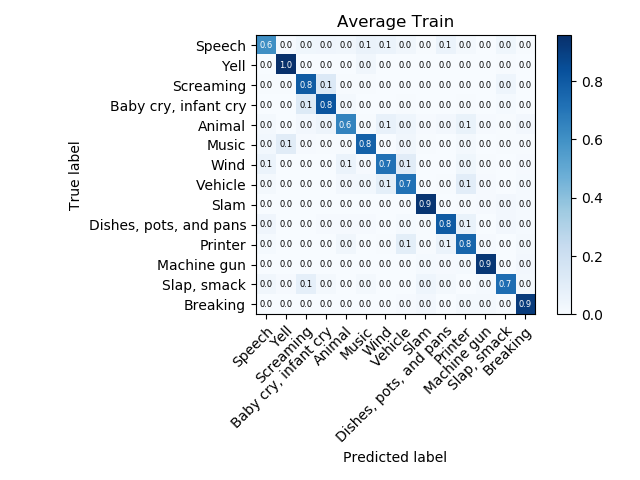
\includegraphics[width=0.6\linewidth]{lstm-multi-cm-tr-av}%
			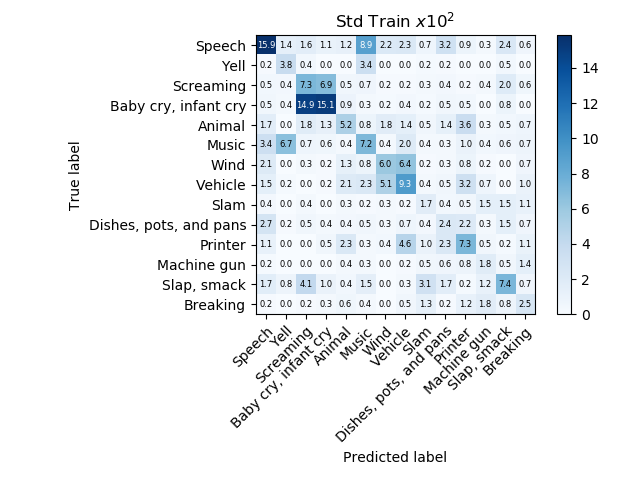
\includegraphics[width=0.6\linewidth]{lstm-multi-cm-tr-std}
			\subcaption{Average and standard deviation for the train set}
		\end{subfigure}
		\vskip\baselineskip
		% Start with figure tfrecord
		\begin{subfigure}[b]{\textwidth}
			\centering
			\captionsetup{justification=centering}
			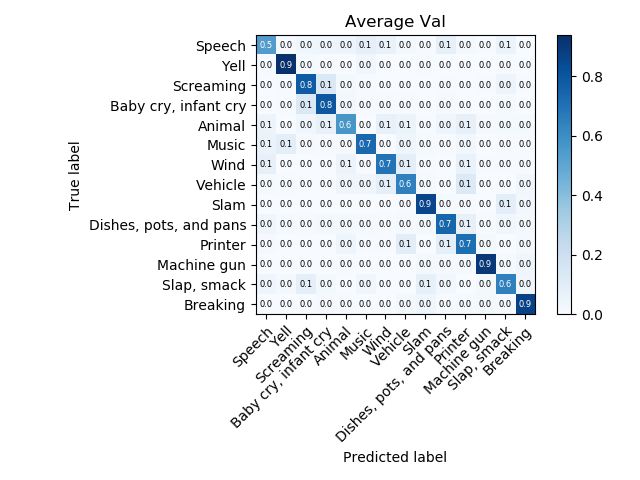
\includegraphics[width=0.6\linewidth]{lstm-multi-cm-val-av}%
			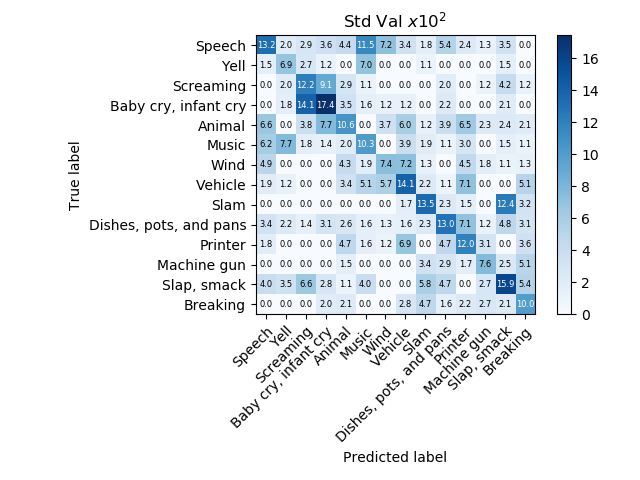
\includegraphics[width=0.6\linewidth]{lstm-multi-cm-val-std}
			\subcaption{Average and standard deviation for the validation set}
		\end{subfigure}
		\caption{Confusion matrices for LSTM multiclass classification for train and validation sets}
		\label{fig:mesh27}
	\end{figure}
	
	\begin{figure}[t]
		\centering
		\captionsetup{justification=centering}
		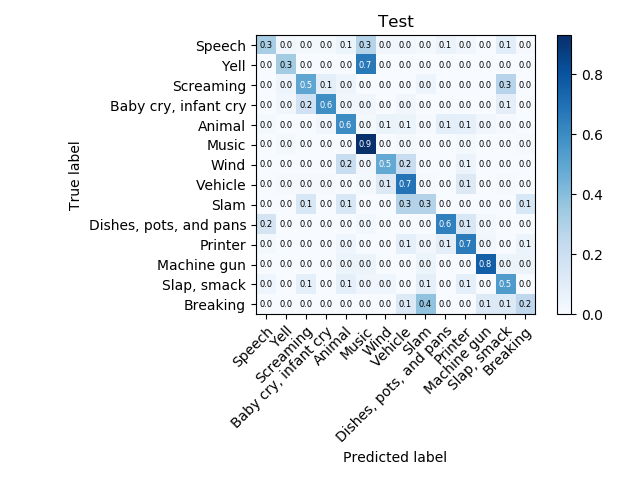
\includegraphics[width=0.7\linewidth]{lstm-multi-cm-tst}
		\caption{Confusion matrix for the test set for the LSTM multiclass classification}
		\label{fig:mesh28}
	\end{figure}
	
	\begin{figure}[t]
		\centering
		\captionsetup{justification=centering}
		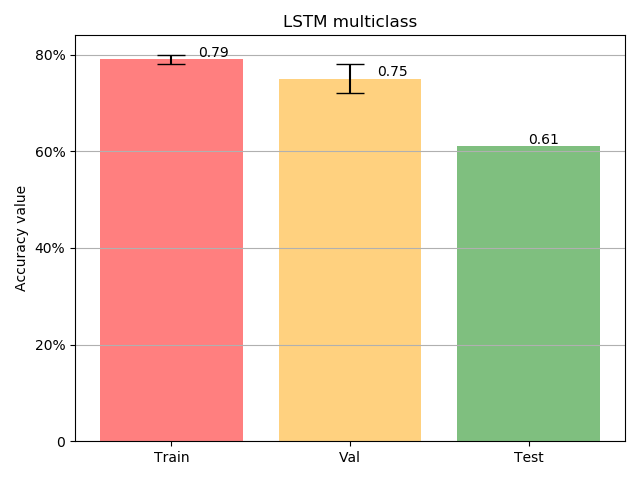
\includegraphics[width=0.7\linewidth]{lstm-multierrorbar}
		\caption{Accuracy values for the three sets for the LSTM multiclass classification}
		\label{fig:mesh29}
	\end{figure}

	For this model, we obtained an accuracy of $79\% \pm 1\%$ for the training set, a $75\% \pm 3\%$ for the validation and a $61\%$ for the test. This can be due to the possible confusion regions mainly between classes such as \textit{Screaming} and \textit{Baby cry, infant cry}, and \textit{Wind} and \textit{Vehicle}, whose standard deviation values are the most emphasized. In the testing procedure, a really good performance was done for the class \textit{Yell}. The other violent classes have a less number of correct predictions but also due to the less amount of samples that belong to these classes in the test subset. There are no signs of overfitting since the values of accuracy in the training and validation sets with respect to the test one are not really away from each other.
	
\subsection{Implementation 4: \acrshort{lstm} multiclass + \acrshort{svm} for a final binary classification}
	
	For this case, the predicted probabilities obtained from the \acrshort{lstm} multiclass classifier as passed as input to the \acrshort{svm} for the binary classification. 
	
	The accuracy value for the different sets are included. Figure \ref{fig:mesh30} shows the average confusion matrices for the train and validation sets. In figure \ref{fig:mesh31}, the confusion matrix for the test set is also included, and in figure \ref{fig:mesh32}, the error bar can be seen with the accuracy values for each of the sets.
	
	\begin{figure}[t]
		\centering
		\captionsetup{justification=centering}
		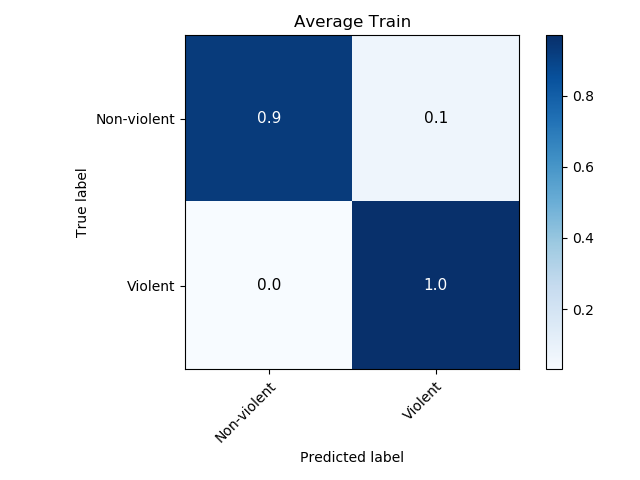
\includegraphics[width=0.6\linewidth]{lstm-svm-cm-tr-av}%
		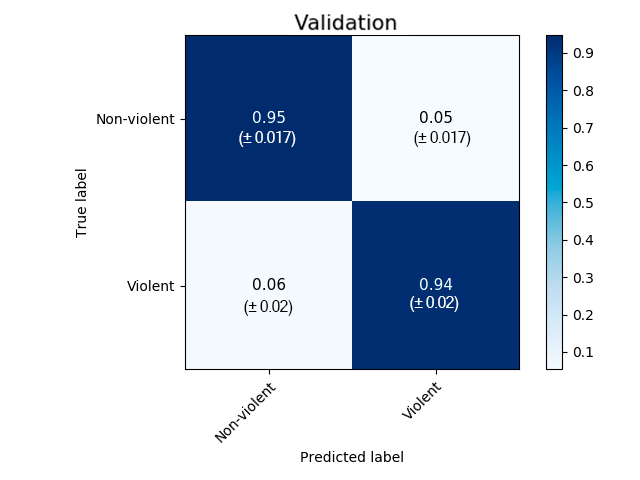
\includegraphics[width=0.6\linewidth]{lstm-svm-cm-val-av}	
		\caption{Average confusion matrices for train and validation in the LSTM multiclass + SVM binary classification}
		\label{fig:mesh30}
	\end{figure}
	
	\begin{figure}[t]
		\centering
		\captionsetup{justification=centering}
		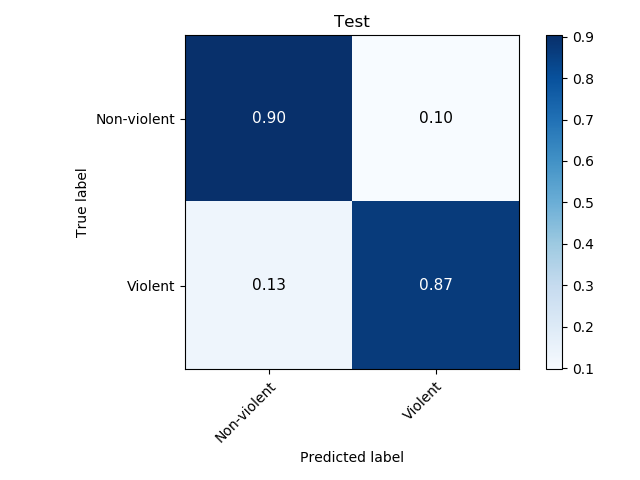
\includegraphics[width=0.7\linewidth]{lstm-svm-cm-tst}
		\caption{Confusion matrix for the test set for the LSTM multiclass + SVM binary classification}
		\label{fig:mesh31}
	\end{figure}
	
	\begin{figure}[t]
		\centering
		\captionsetup{justification=centering}
		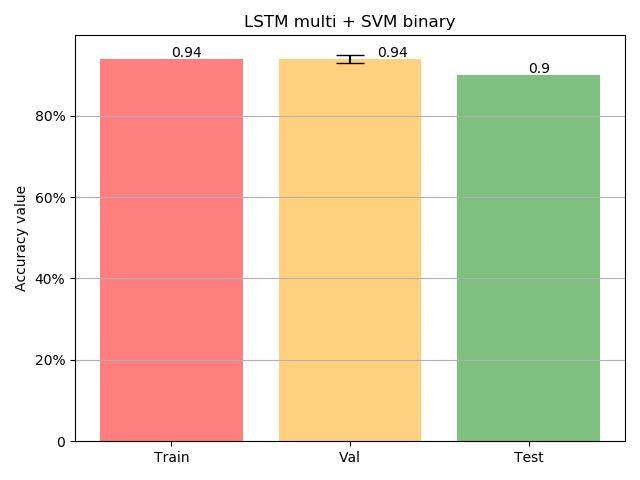
\includegraphics[width=0.7\linewidth]{lstm-svmerrorbar}
		\caption{Accuracy values for the three sets for the LSTM multiclass + SVM binary classification}
		\label{fig:mesh32}
	\end{figure}

	
\subsection{Implementation 5: \acrshort{cnn} for multiclass classification}

	For this case, we have implemented a \acrshort{cnn} model based on the architecture presented in figure \ref{fig:mesh5} in subsection \ref{subsection:exploring-differences-between-two-types-of-data-access} for the small experiment to check the similarity of the embeddings from the .\textit{tfrecord} files and the naturally audio files.
	
	In the configuration of the network, the same hyperparameters from implementation 3 are used for the learning process: a categorical cross-entropy for the loss function, a \acrshort{nadam} optimizer, a number of 50 epochs and a batch size of 32 samples. We have kept the same value for this model since the number of observations is the same and the depth of the network is not very great. A learning rate of $2e^{-3}$ was also used. 
	
	In figure \ref{fig:mesh33}, the average and standard deviation matrices for the train and validation sets are shown. In figure \ref{fig:mesh34}, the confusion matrix for the test set. The bar plot in \ref{fig:mesh35}, shows the accuracy for every set with their standard deviation values.
	
	\begin{figure}[ht]
		% Whole figure
		\captionsetup{justification=centering}
		\begin{subfigure}[b]{\textwidth}
			\centering
			% Start with figure wav
			\captionsetup{justification=centering}
			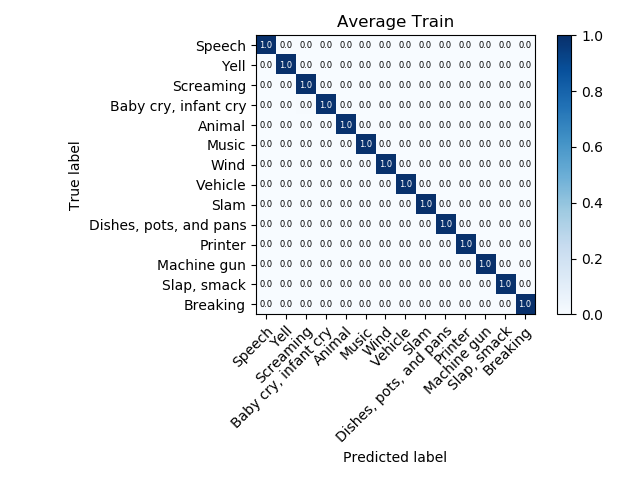
\includegraphics[width=0.6\linewidth]{cnn-multi-cm-tr-av}%
			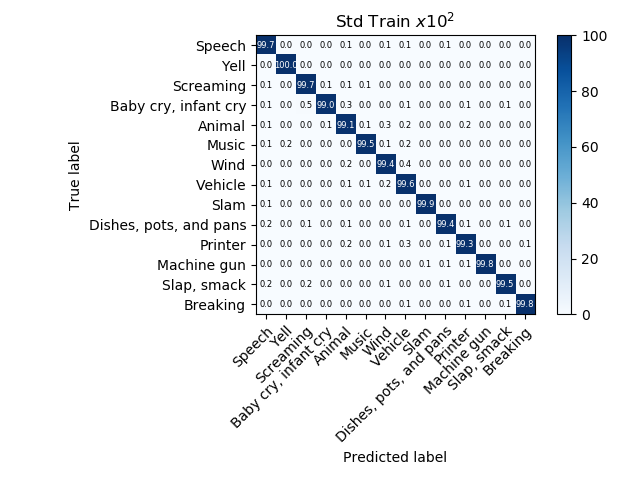
\includegraphics[width=0.6\linewidth]{cnn-multi-cm-tr-std}
			\subcaption{Average and standard deviation for the train set}
		\end{subfigure}
		\vskip\baselineskip
		% Start with figure tfrecord
		\begin{subfigure}[b]{\textwidth}
			\centering
			\captionsetup{justification=centering}
			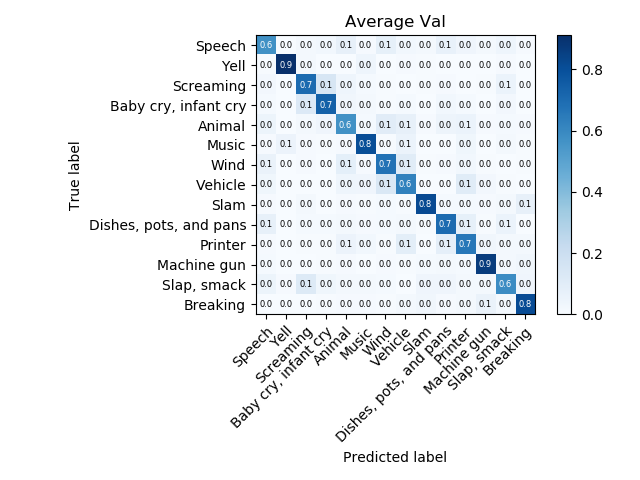
\includegraphics[width=0.6\linewidth]{cnn-multi-cm-val-av}%
			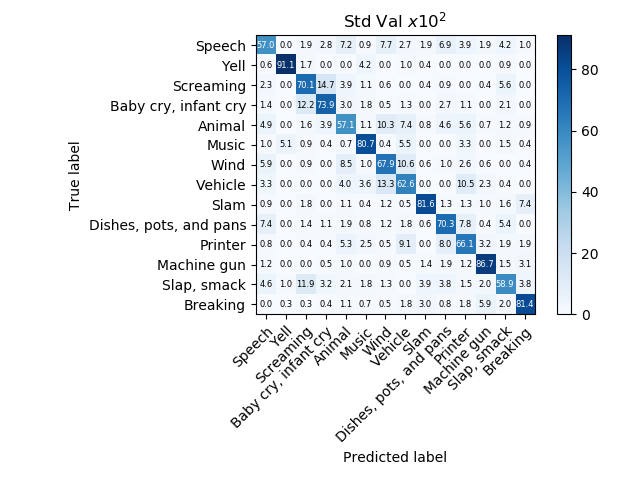
\includegraphics[width=0.6\linewidth]{cnn-multi-cm-val-std}
			\subcaption{Average and standard deviation for the validation set}
		\end{subfigure}
		\caption{Confusion matrices for CNN multiclass classification for train and validation sets}
		\label{fig:mesh33}
	\end{figure}
	
	\begin{figure}[t]
		\centering
		\captionsetup{justification=centering}
		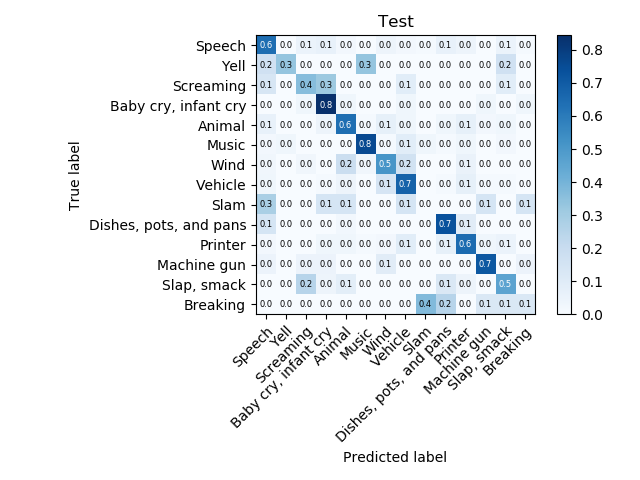
\includegraphics[width=0.7\linewidth]{cnn-multi-cm-tst}
		\caption{Confusion matrix for the test set for the CNN multiclass classification}
		\label{fig:mesh34}
	\end{figure}
	
	\begin{figure}[t]
		\centering
		\captionsetup{justification=centering}
		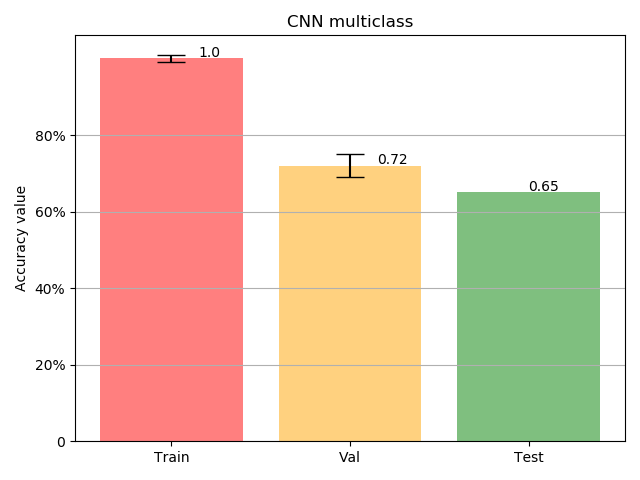
\includegraphics[width=0.7\linewidth]{cnn-multierrorbar}
		\caption{Accuracy values for the three sets for the CNN multiclass classification}
		\label{fig:mesh35}
	\end{figure} 

\subsection{Implementation 6: \acrshort{cnn} multiclass + \acrshort{svm} for a final binary classification}

	In this last approach we wanted to use the predictions from the \acrshort{cnn} to feed the binary classifier \acrshort{svm}.
	
	In figure \ref{fig:mesh36} shows the average of the confusion matrices for the train and validation sets. In figure \ref{fig:mesh37}, it is included the confusion matrix for the test set. Finally, figure \ref{fig:mesh38} shows the error bar in which the accuracy values for the three test can be seen.
	
	\todo{Still doing an execution to get the plots}
	
	\begin{figure}[t]
		\centering
		\captionsetup{justification=centering}
		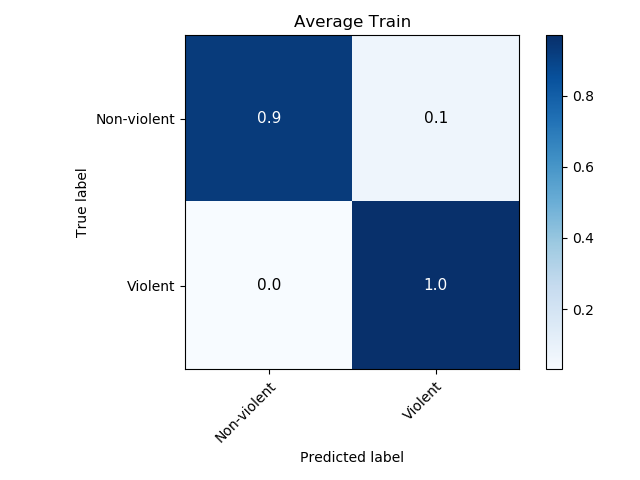
\includegraphics[width=0.6\linewidth]{lstm-svm-cm-tr-av}%
		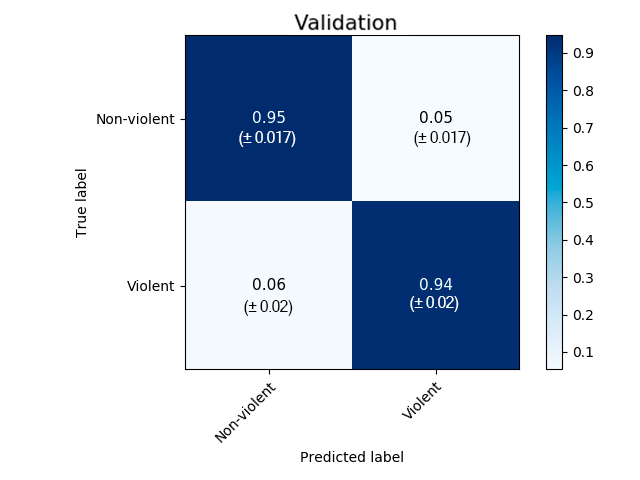
\includegraphics[width=0.6\linewidth]{lstm-svm-cm-val-av}	
		\caption{Average confusion matrices for train and validation in the CNN multiclass + SVM binary classification}
		\label{fig:mesh36}
	\end{figure}
	
	\begin{figure}[t]
		\centering
		\captionsetup{justification=centering}
		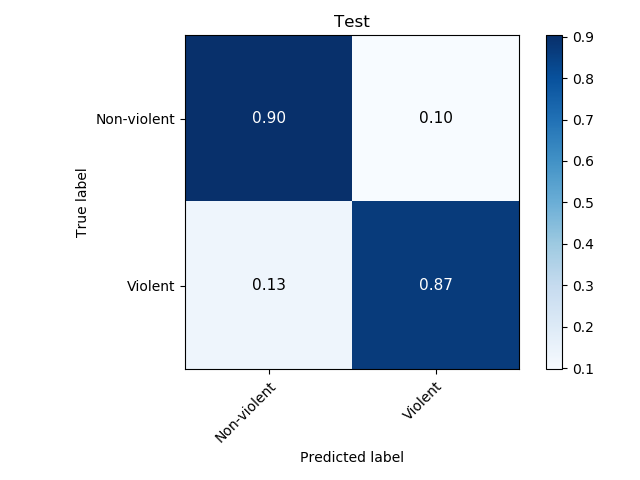
\includegraphics[width=0.7\linewidth]{lstm-svm-cm-tst}
		\caption{Confusion matrix for the test set for the CNN multiclass + SVM binary classification}
		\label{fig:mesh37}
	\end{figure}
	
	\begin{figure}[t]
		\centering
		\captionsetup{justification=centering}
		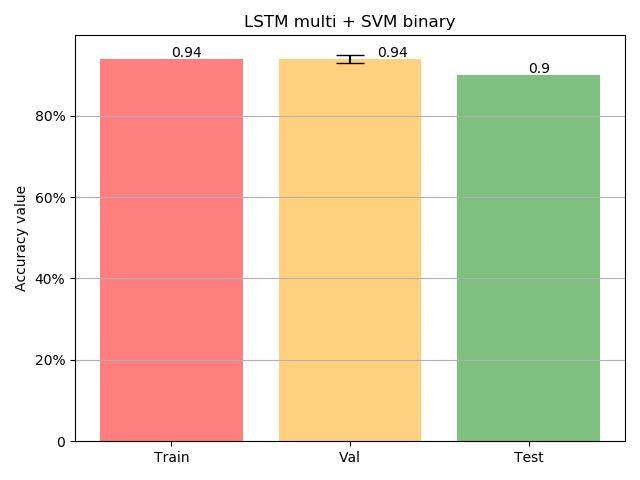
\includegraphics[width=0.7\linewidth]{lstm-svmerrorbar}
		\caption{Accuracy values for the three sets for the CNN multiclass + SVM binary classification}
		\label{fig:mesh38}
	\end{figure}
	
	